In all we have done so far in this unit, we have assumed that the input was deterministic: the algorithm is randomised, yes, but the input itself is fixed, and arbitrary.

In this lecture, we (somewhat) change this. What we have is access to a sequence of independent, identically distributed (\iid) data points, coming from an \emph{unknown} probability distribution $\p$:
\[
    x_1,\dots, x_\ns \sim \p
\]
and what we want to do is to \emph{learn something about this $\p$}. Put differently:
\begin{framed}
    \noindent The input is not the \iid sequence $(x_1,\dots, x_\ns)$: the input is $\p$, and  $x_1,\dots, x_\ns$ is how we get to access this input.
\end{framed}
We will make very few assumptions about this unknown probability distribution $\p$: except that it is over a known \emph{discrete} domain $\domain$ of size $\abs{\domain} = \ab$. 

To illustrate this, here is a histogram, corresponding to the counts from $\ns=3665$ \iid\ draws\marginnote{\emph{Presumably} \iid} from some unknown probability distribution $\p$ over $\domain = \{1,2,\dots,49\}$ of size $\ab=49$. They correspond to a number drawn, every week from 1982 to 2018, from Canada's ``Lotto 6/49'':
\begin{figure}[htbp]
    \centering
    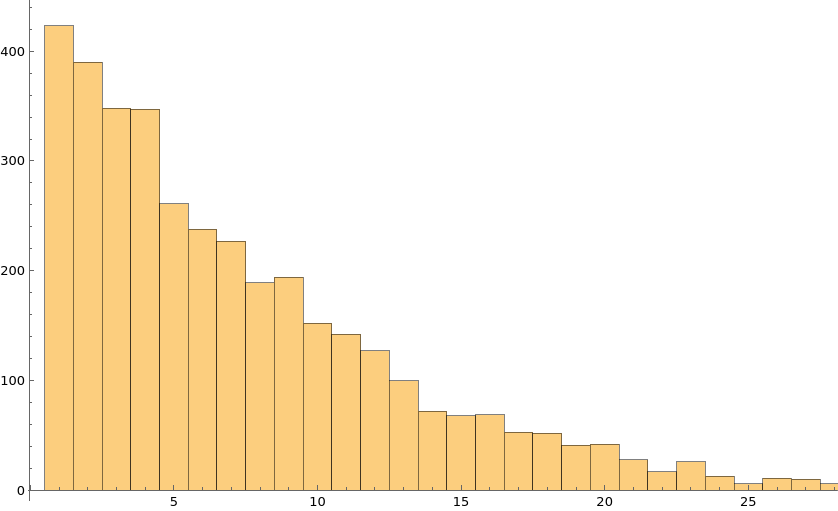
\includegraphics[width=0.925\linewidth]{figures/fig-lotto-minofsix.png}
    \caption{Counts for each of the $\ab=49$ possible numbers among the $\ns=3665$ draws. What is distribution $\p$ does this correspond to? (Data from the Kaggle ``Lotto 649'' dataset.)}
    \label{fig:enter-label} % Min of 6 uniform
\end{figure}
\noindent Here are some questions we may want to answer about $\p$:
\begin{itemize}
    \item \emph{What is it?} That is, can we \emph{learn} the whole unknown probability distribution?
    \item \emph{What are some of its characteristics?} That is, can we \emph{learn} some ``simple'' parameter $f(\p)$, such as its mean, entropy, variance?
    \item \emph{Does it satisfy some specific property?} That is, can we \emph{test} if $\p$ satisfies some requirement we care about? For instance, in the case of the lotto numbers above, ``{is $\p$ consistent with the distribution of the minimum of 6 independent uniform random numbers in $\{1,2,\dots, 49\}$?}''
\end{itemize}
Intuitively, we can think of the first as learning $\approx \ab$ values about $\p$, the second as learning \emph{one} value, and the last one as learning \emph{one bit}. So presumably, they should be in decreasing order of ``complexity,'' for whatever notion of ``complexity'' we define.


\paragraph{What is the notion of complexity?} Our algorithms, as mentioned about, can only access the input $\p$ through queries which give\marginnote{Think of $\ns$ as the size of the dataset you need to collect, or generate, or buy in order for your algorithm to succeed. In the case of the lotto example, the number of observations is limited: there is only one lotto every week, we cannot choose $\ns$ to be as large as we want.} \emph{independent, identically distributed} samples from $\p$. We will of course care about the running time of the algorithms, but our main objective  will be to minimise the number $\ns$ of queries we make.

\paragraph{What is the randomness?} Since what we feed to the algorithm, the sequence of samples $x_1,\dots, x_\ns$, is random, there will always be some probability our algorithm's output is wrong. That is, now, when we discuss expectations and probabilities, it will be over (1)~the randomness of the algorithm itself, as usual, but also (2)~the randomness in drawing $x_1,\dots, x_\ns$ from the unknown $\p$.

\paragraph{What are the parameters?} Of course, the domain size, $\ab$, is a key 
parameter of the problem. But we have at least two others: first, the probability of failure, $\errprob$: we want the algorithm to be correct about $\p$ most of the time. The other will be a \emph{distance parameter}, $\dst >0$: we will get back to this soon, as its meaning depends on which of the three problems we are interested in. But overall, our goal will be:
\begin{framed}
    Find the smallest value $\ns = \ns(\ab, \dst, \errprob)$ for which an algorithm can solve the learning, estimation, or testing task we care about with distance parameter $\dst$ and failure probability at most $\errprob$. 
\end{framed}

\paragraph{Some notation} A probability distribution over $\domain$ can be identified to its probability mass function (pmf), which is a function $\p\colon\domain\to [0,1]$ such that $\sum_{x\in \domain}\p(x) = 1$. Accordingly, the probability mass that $\p$ assigns to a subset\footnote{As we only consider discrete domains, we ignore issues of measurability, etc. That is, we consider $\domain$ endowed with the counting measure, so every set is measurable. What is discussed here generalises to continuous probability distributions, but with annoying technical details.} $S\subseteq \domain$ is $\p(S) = \sum_{x\in S} \p(x) = \probaDistrOf{x\sim\p}{x\in S}$. Finally, $\distribs{\domain}$ denotes the set of all probability distributions over our domain $\domain$.

\section{Distance between probability distributions}
To define what it means to learn a probability distribution, or even how \emph{far} two probability distributions over the same domain $\domain$ are, we need a notion of \emph{distance}. Ideally, one which makes ``sense'': (1)~a metric would be nice (to be able to use the triangle inequality when needed), (2)~a \emph{bounded} metric would be even nicer (to be able to understand a value such as $0.1$ without having to normalise or think twice), (3)~a bounded metric \emph{with a simple and meaningful interpretation} would be best.

This leads us to the the notion of distance we will be concerned about, the total variation distance (also known as \emph{statistical distance}).
\begin{definition}[Total variation distance]
  \label{def:tv}
  The \emph{total variation distance} between two probability distributions $\p,\q\in\distribs{\domain}$ is given by
  \[
    \totalvardist{\p}{\q} = \sup_{S\subseteq \domain} (\p(S)-\q(S))\,.
  \]
  Given a subset $\class\subseteq\distribs{\domain}$ of distributions, we further define the distance from $\p\in\distribs{\domain}$ to $\class$ as $\totalvardist{\p}{\class} \eqdef \inf_{\q\in\class} \totalvardist{\p}{\q}$, and will say that $\p$ is \emph{$\dst$-far from $\class$} if $\totalvardist{\p}{\class} > \dst$.
\end{definition}
One can check\marginnote{Check it!} that $\dtv$ defines a metric on $\distribs{\domain}$, and takes values in $[0,1]$. Moreover, the total variation distance exhibits several important properties, among which one of the most important is its \emph{immunity to post-processing}:
\begin{fact}[Data Processing Inequality]
  \label{fact:dpi}
  Suppose $X$ and $Y$ are independent random variables with distributions $\p$ and $\q$, and let $f$ be any (possibly randomized) function independent of $X,Y$. Then the probability distributions $\p_f$ and $\q_f$ of $f(X)$ and $f(Y)$ satisfy
  \[
      \totalvardist{\p_f}{\q_f} \leq \totalvardist{\p}{\q}\,.
  \]
  That is, \emph{postprocessing cannot increase the total variation distance.}
\end{fact}
What this says is, paraphrasing, that post-processing two random variables the same way cannot ``make them statistically farther.''


%%%%%%%%%%%%%%%%%%%%%%%%%%%
Interestingly, total variation distance also has a very natural interpretation in terms of \emph{indistinguishability}:
\begin{lemma}[Pearson--Neyman]
  \label{lemma:pearsonneyman}
  Any (possibly randomized) algorithm which distinguishes between $\p$ and $\q$ from a \emph{single} sample must have Type~I (false positive) and Type-II (false negative) errors satisfying
  \[
      \text{Type~I} + \text{Type~II} \geq 1- \totalvardist{\p}{\q}
  \]
  Moreover, this is achieved by the test which outputs ``$\q$'' if, and only if, the sample belongs to the ``Scheff\'e set'' $S^\ast \eqdef \setOfSuchThat{x}{\q(x) > \p(x)}$.
\end{lemma}
\begin{proof}\marginnote{You can ignore the proof in a first read, it is just here for completeness. What matters is the lemma itself.}
Fix any test $\Algo$ distinguishing between two distributions $\p$ and $\q$, given a single observation. Letting $\alpha$ and $\beta$ denote the Type~I and Type-II errors of $\Algo$, we have
\begin{align*}
  \alpha+\beta 
  &= \probaDistrOf{\p,R}{\Algo(X,R)=1} + \probaDistrOf{\q,R}{\Algo(X,R)=0} \\
  &= \shortexpect_{R}[ \probaDistrOf{\p}{\Algo(X,R)=1} ] + \shortexpect_{R}[ \probaDistrOf{\q}{\Algo(X,R)=0} ] \\
  &= \shortexpect_{R}[ \probaDistrOf{\p}{\Algo(X,R)=1} + \probaDistrOf{\q}{\Algo(X,R)=0} ]
%   \totalvardist{\p}{\q}
\end{align*}
where we denote by $R$ the internal randomness of $\Algo$. Since, for any fixed realization $r$ of this randomness $R$, the resulting test $\Algo(\cdot,r)$ is deterministic, we can define for any $r$ the \emph{acceptance region} $S_{\Algo,r} \eqdef \setOfSuchThat{x}{\Algo(x,r)=1}$, and write
\begin{align*}
  \alpha+\beta 
  &= \shortexpect_{R}[ \probaDistrOf{\p}{X \in S_{\Algo,R}} + \probaDistrOf{\q}{X \notin S_{\Algo,R}} ] \\
  &= 1+\shortexpect_{R}[ \p(S_{\Algo,R}) - \q(S_{\Algo,R}) ] \\
  &\geq 1 + \inf_{S}(\p(S) - \q(S)) \\
  &= 1 - \sup_{S}(\q(S) - \p(S)) \\
  &= 1- \totalvardist{\p}{\q}\,,
\end{align*}
as claimed. Finally, it is immediate from the definition of total variation distance that the proposed test satisfies $\text{Type~I} + \text{Type~II} = 1 + \p(S^\ast) - \q(S^\ast) = 1- \totalvardist{\p}{\q}$.
\end{proof}
%%%%%%%%%%%%%%%%%%%%%%%%%%%
Here is one way to interpret this lemma: 
\begin{framed}
Alice and Bob play a game, where they both know two probability distributions $\p,\q$. Alice starts by tossing a fair coin, and does not show the outcome to Bob: if it is \textsf{Heads}, then she draws $x\sim \p$; if it is \textsf{Tails}, she draws $x\sim \q$. Then she shows the value of $x$ to Bob, who must guess if the coin toss was \textsf{Heads}.
Clearly, just by random guessing, Bob can win the game with probability $1/2$. What the lemma says is that he can do better: there is a strategy for him to win with probability
\[
    \probaOf{\text{Bob wins}} = \frac{1}{2}+\frac{\totalvardist{\p}{\q}}{2}
\]
and, moreover, this is the best possible.
\end{framed}
One more (very useful) fact about total variation distance: it is just $\lp[1]$ distance in disguise!
\begin{fact}[Scheff\'e's Lemma]
\label{fact:scheffe}
For any two $\p,\q\in\distribs{\ab}$,
  \begin{equation}
    \label{eq:tv:l1}
    \totalvardist{\p}{\q} = \frac{1}{2}\sum_{x\in\domain} \abs{\p(x)-\q(x)} = \frac{1}{2}\normone{\p-\q}
  \end{equation}
  that is, ``total variation is half the $\lp[1]$ distance between pmfs.''
\end{fact}
This fact, which you will prove during the tutorial, turns out to be a very useful connection: if nothing else, $\lp[p]$ norms are well studied, and this will allow us to use our arsenal of geometric inequalities --- H\"older, Cauchy--Schwarz, and monotonicity of $\lp[p]$ norms, to name a few.

\section{The case of a coin ($\ab=2$)}
With the necessary background in hand, we can look at our first question: forget for now about $\ab \gg 1$, let us focus on the simplest, most basic case, $\ab=2$: you are given \emph{a coin}, and it may be biased.

The learning task can be then rephrased as follows:
\begin{framed}
    How many times $\ns$ do you need to flip the coin to learn its true bias $p$ to accuracy $\pm\dst$, and be correct with probability at least $1-\errprob$?
\end{framed}
\noindent Should it be\dots
\begin{itemize}
    \item $\ns = \bigO{\frac{1}{\dst\errprob}}$ times?
    \item $\ns = \bigO{\frac{1}{\dst^2\errprob}}$ times?
    \item $\ns = \bigO{\frac{1}{\dst^2}\log\frac{1}{\errprob}}$ times?
    \item $\ns = \bigO{\frac{1}{\dst}\log\frac{1}{\errprob}}$ times?
\end{itemize}
Well, actually, we can get something more refined than any of the bounds above! If we are given a promise on the unknown bias $p$, then we can get the following:
\begin{theorem}
    Suppose we are promised that the true bias $p$ of the coin satisfies $0\leq p < q \leq \frac{1}{2}$, for some known value $q$. Then estimating the bias of the coin to an additive $\dst$, with probability at least $1-\errprob$, can be done with $\ns = \bigO{\frac{q}{\dst^2}\log\frac{1}{\errprob}}$ \iid samples. (Moreover, this is optimal.)
\end{theorem}
\begin{proof}
    This follows from a Chernoff bound, using the empirical estimate
    \[
        \hat{p} \eqdef \frac{1}{\ns}\sum_{i=1}^\ns x_i
    \]
    where $x_1, \dots, x_\ns \sim \bernoulli{p}$.
    Note that a Hoeffding bound would not give you the dependence on $q$. (The lower bound, \ie proof of optimality, is beyond the scope of this lecture.)
\end{proof}
As a remark, the assumption that $q \in(0,1/2]$ is without loss of generality: if instead we were promised that $q < p \leq 1$ with $q \in (1/2, 1)$, then we could flip the coin flips (!) by looking at $x'_i \eqdef 1-x_i$ instead, and estimate the bias $p' \eqdef 1-p$, which satisfies $0 \leq p' < 1-q \leq 1/2$. Clearly, estimating $p'$ to $\pm\dst$ is equivalent to estimate $p$ to $\pm \dst$.
\begin{corollary}
    \label{theo:learning:bias}
    Estimating the bias of a coin to an additive $\dst$, with probability at least $1-\errprob$, can be done with $\ns = \bigO{\frac{1}{\dst^2}\log\frac{1}{\errprob}}$ \iid samples. (Moreover, this is optimal.)
\end{corollary}
This follows from applying the above theorem setting $q=1/2$; alternatively, the upper bound can be directly proven using the Hoeffding bound.\marginnote{Try it!}

This is if we want to \emph{learn} the bias of an unknown coin. What if we just want to \emph{test} if it is biased? That is, distinguish between the case where (1)~the coin is \textsf{Heads} with probability exactly $1/2$ (fair coin), or probability $1/2 \pm \Omega(\dst)$ (biased coin)? How many times $\ns$ would we have to toss the coin, if we wanted our diagnostic to be correct with probability at least $1-\errprob$?
\begin{itemize}
    \item $\ns = \bigO{\frac{1}{\dst}\sqrt{\log\frac{1}{\errprob}}}$ times?
    \item $\ns = \bigO{\frac{1}{\dst^2}\sqrt{\log\frac{1}{\errprob}}}$ times?
    \item $\ns = \bigO{\frac{1}{\dst^2}\log\frac{1}{\errprob}}$ times?
    \item $\ns = \bigO{\frac{1}{\dst}\log\frac{1}{\errprob}}$ times?
\end{itemize}
As it turns out\dots \emph{testing} whether the coin is biased or fair is basically as hard as \emph{learning} the bias of the coin:
\begin{theorem}
    \label{theo:testing:bias:basic}
    Testing whether the bias of a coin is $1/2$ or at least $1/2+\dst$, with probability at least $1-\errprob$, can be done with $\ns = \bigO{\frac{1}{\dst^2}\log\frac{1}{\errprob}}$ \iid samples. (Moreover, this is optimal.)
\end{theorem}
This is a little underwhelming, since one can literally do this by learning the bias up to $\frac{\dst}{2}$.\footnote{Can you see how?} And that provides a lot more information! So is there anything to be gained (except maybe constant factors) if we only want to test tthe bias of the coin? As it turns out, \emph{yes}\dots but not always. \emph{Not} when testing if a coin is fair or biased: but when testing if the coin is very biased or \emph{extremely} biased, then yes.
\begin{theorem}
\label{theo:testing:bias:refined}
    For any $0 <\purple{\alpha} \leq 1/2$ and $\dst\in(0,1]$, testing whether the bias of a coin is at most $\purple{\alpha}$ or at least $\purple{\alpha}(1+\dst)$, with probability at least $1-\errprob$, can be done with $\ns = \bigO{\frac{1}{\purple{\alpha}\dst^2}\log\frac{1}{\errprob}}$ \iid samples.
\end{theorem}
Again, this is not very useful when $\purple{\alpha} = \Omega(1)$: however, for vanishing $\purple{\alpha}$, this is much better than what learning the bias to an additive $\pm \frac{1}{2}\purple{\alpha}\dst$ would give, which by~\cref{theo:learning:bias} is $\ns= \bigO{\frac{1}{\purple{\alpha}^2\dst^2}\log\frac{1}{\errprob}}$.

\cref{theo:testing:bias:refined} can be proven by a Chernoff bound, specifically the version given in~\cref{theo:chernoff:with:ublb} applied to the same empirical estimator $\hat{p}$. But rather than \emph{proving} it, let us give a small sketch of \emph{why} we could expect this statement to be true, to get some intuition (and remember the result). If the true bias $p$ is roughly $\Theta(\purple{\alpha})$, then we expect to see \textsf{Tails} most of the time, and \textsf{Heads} a $\Theta(\purple{\alpha})$ fraction of the tosses. That is, in every chunk of $1/\purple{2\alpha}$ tosses, we expect to see a \textsf{Heads} with probability either at most $1/2$ (if $p \leq \purple{\alpha}$) or at least $(1+\dst)/2$ (if $p \geq (1+\dst)\purple{\alpha}$). But by~\cref{theo:testing:bias:basic} (ignoring $\errprob$ for simplicity), this takes $\bigO{{1}/{\dst^2}}$ chunks~--~so $\bigO{{1}/{(\purple{\alpha}\dst^2)}}$ coin tosses in total.

\emph{And this makes sense!} Things should become easier in the ``highly biased'' regime. With a similar analysis, one can show that distinguishing between bias $p=0$ and bias $p\geq \dst$ takes only $\ns=O(1/\dst \log(1/\errprob))$ coin tosses. And this is easy to interpret: in one case, you \emph{never} see a \textsf{Heads}, and in the other, you will see one after $\approx 1/\dst$ coin tosses. What is really hard (and requires more coin tosses) is when $p\approx 1/2$, and you have to distinguish between ``a lot of \textsf{Heads}'' and ``a lot of \textsf{Heads}, \emph{but slightly more}.''

\section{Learning and testing beyond coins}
This is all well and good, but we often have to consider data over domains of size $\ab \gg 2$. The lotto example above, for instance, was for $\ab = 49$; and that's only for \emph{one} number: if one considers all 6 draws in a single ticket of that Canadian lotto, that's a domain of size $\ab = 49^6 = 13,841,287,201$.

If we were given an algorithm to generate random permutations and we wanted to test whether its output was truly uniform (on the space of all permutations of, say, size $8$), then we would be looking at a space of size $16! = 209,22,789,888,000$.

If we wanted to estimate the entropy of a dataset of $8$-character passwords made of lower and uppercase letters, digits, and special characters $\$\%\#\&!?\_-$, then $\ab = (70)^{8} = 576,480,100,000,000$. 
\begin{framed}
Domain sizes grow quite fast, and in most settings $\ab$ is huge.
\end{framed}
If we cannot assume structure in the data, then we have to hope for \emph{very} sample-efficient algorithms.

\section{Learning}
In \emph{learning} (in total variation distance),\footnote{One can define learning with respect to other notions of distances: \eg Kullback--Leibler divergence, or $\lp[\infty]$ distance. Here we focus on the standard, nice, total variation.} our goal is to design an algorithm $\Algo$ which, given $\ns$ \iid samples from $\p$ and parameters $\dst,\errprob\in(0,1]$, outputs $\widehat{\p}$ such that
\begin{equation}
    \probaOf{ \totalvardist{\p}{\widehat{\p}} > \dst } \leq \errprob
\end{equation}
that is, $\widehat{\p}$ is close to $\p$, with high probability. The probability is taken, again, over both the samples $x_1,\dots, x_{\ns}\sim \p$ \emph{and} the randomness of the algorithm $\Algo$.

How many samples $\ns$ would we have to take, if we wanted the output $\widehat{\p}$ to be $\dst$-close to the true $\p$ with probability at least $1-\errprob$?
\begin{itemize}
    \item $\ns = \bigO{\frac{\ab^2}{\dst}\log\frac{1}{\errprob}}$?
    \item $\ns = \bigO{\frac{\ab}{\dst^2}\log\frac{1}{\errprob}}$?
    \item $\ns = \bigO{\frac{\ab + \log\frac{1}{\errprob}}{\dst^2}}$?
    \item $\ns = \bigO{\frac{\ab^2 + \log\frac{1}{\errprob}}{\dst^2}}$?
\end{itemize}
As we will see, the answer is not entirely obvious, even though the algorithm $\Algo$ is. 

\paragraph{First idea: using what we saw}
We want to estimate all $\ab$ probabilities $\p_1,\dots, \p_{\ab}$ to get $\widehat{\p}_1,\dots,\widehat{\p}_{\ab}$ such that
\[
    \frac{1}{2}\sum_{i=1}^{\ab} \abs{\widehat{\p}_i-\p_i} \leq \dst\,.
\]
It would be \emph{enough} to estimate each individual $\p_i$ to an additive $\frac{2\dst}{\ab}$.\footnote{Ignore for now the fact that doing so, we may not have $\sum_{i=1}^{\ab} \widehat{\p}_i = 1$: we can normalise afterwards.} To make sure we learn \emph{all} $\ab$ of them, we will learn each with error failure $\frac{\errprob}{\ab}$ and take a union bound.

The total cost, from~\cref{theo:learning:bias}, is then
\begin{equation}
\ns = \bigO{ \frac{1}{(\dst/\ab)^2} \log\frac{1}{(\errprob/\ab)} }
= \bigO{ \frac{\ab^2}{\dst^2}\log\frac{\ab}{\errprob} }\,.
\end{equation}
That's something, but that has a more-than-\emph{quadratic} dependence on this giant parameter $\ab$. \smallskip

\emph{But we can do better!} Another idea would be to learn each $\p_i$ to a multiplicative factor $(1\pm 2\dst)$, instead of an additive $\pm \frac{2\dst}{\ab}$. \emph{If} we assume that $\p_i \geq \frac{\dst}{\ab}$ for all $1\leq i\leq \ab$, for instance, then a Chernoff bound (along with a union bound) tell us that we can the empirical estimates $\hat{\p}_1,$ satisfy
\[
    (1- 2\dst)\p_i \leq \widehat{\p}_i \leq (1+2\dst)\p_i, \text{ for all } 1\leq i\leq \ab
\]
with probability at least $1-\errprob$, for
\begin{equation}
    \ns = \bigO{ \frac{\ab}{\dst^3}\log\frac{\ab}{\errprob} }
\end{equation}
and then
\[
    \frac{1}{2}\sum_{i=1}^{\ab} \abs{\widehat{\p}_i-\p_i} \leq \frac{1}{2}\sum_{i=1}^{\ab} 2\dst \p_i = \dst\,,
\]
since $\sum_{i=1}^{\ab} \p_i = 1$. Moreover, we can get rid of that assumption on $\min_i \p_i$, losing only constant factors in the final bound.\marginnote{$(\star)$ Can you see how? Hint: ``mix'' $\p$ with uniform, and learn \[
\p' = (1-\frac{\dst}{2})\p + \frac{\dst}{2}\uniform_{\ab}
\]instead, where $\uniform_{\ab}$ is the uniform distribution on $\domain$.}\medskip

\emph{But we can do better!} One of the two bounds above has a (near) quadratic dependence on $\ab$ but a quadratic dependence on $1/\dst$, the other is (near) linear in $\ab$ but has a cubic dependence on $1/\dst$, and both have an extra logarithmic factor in $\ab$ because of a union bound. This does not ``feel'' right, and indeed it is not:

\begin{theorem}
    \label{theo:learning:k}
    Learning an unknown distribution $\p\in\distribs{\ab}$ to total variation distance $\dst$ (with success probability $1-\errprob$) can be done with 
    \[
    \ns = \bigO{\frac{\ab + \log\frac{1}{\errprob}}{\dst^2}}
    \]\iid samples. (Moreover, this is optimal.)
\end{theorem}
% Talk about monotonicity in the tutorial?
% DKW?
We will only prove the upper bound statement (not the lower bound showing this sample complexity is optimal), but it is worth noting that we have $\ab+\log(1/\errprob)$, \emph{not} $\ab\log(1/\errprob)$: this is perhaps surprising, as $\ab\log(1/\errprob)$ is what the median trick would give us.
\begin{proof}[Proof of~\cref{theo:learning:k}]
    Consider the empirical distribution $\widehat{\p}$ obtained by drawing $\ns$ independent samples $x_1,\dots,x_\ns$ from the underlying distribution $\p\in\distribs{[\ab]}$:
\begin{equation}\label{def:empirical}
\widehat{\p}(i) = \frac{1}{\ns} \sum_{j=1}^\ns \indic{x_j=i}, \qquad i\in [\ab]
\end{equation}
This defines a valid probability distribution (\ie $\widehat{\p}\in\distribs{\ab}$), and moreover can be computed efficiently, in time $O(\ab+\ns\log\ns)$.

Recalling the definition of total variation distance (\cref{def:tv}), the key observation is that we have $\totalvardist{\p}{\widehat{\p}} > \dst$ if, and only if, there exists a subset $S\subseteq [\ab]$ such that $\widehat{\p}(S) > \p(S) + \dst$. There are only $2^{\ab}$ subsets (actually $2^{\ab}-2$) to consider, so we will make sure our estimate is accurate for \emph{each} subset, taking a union bound over all $2^{\ab}$ of them.

Fix any $S\subseteq[\ab]$. We have
\[
	\widehat{\p}(S) = \sum_{i\in S} \widehat{\p}(i) \operatorname*{=}^{\eqref{def:empirical}} \frac{1}{\ns} \sum_{i\in S} \sum_{j=1}^\ns \indic{x_j=i}
\]
and so, letting $X_j \eqdef \sum_{i\in S}\indic{x_j=i}$ for $j\in [\ns]$, we have
$
\widehat{\p}(S) = \frac{1}{\ns}\sum_{j=1}^\ns X_j
$ where the $X_j$'s are \iid Bernoulli random variables with parameter $\p(S)$. By a Hoeffding bound,
\[
    \probaOf{ \widehat{\p}(S) > \p(S) + \dst } = \probaOf{ \frac{1}{\ns}\sum_{j=1}^\ns X_j > \expect{\frac{1}{\ns}\sum_{j=1}^\ns X_j} + \dst } \leq e^{-2\dst^2 \ns}
\]
and therefore $\probaOf{ \widehat{\p}(S) > \p(S) + \dst } \leq \frac{\errprob}{2^{\ab}}$ as long as
\begin{equation}
\ns\geq \frac{\ab\ln 2+\log(1/\errprob)}{2\dst^2}
\end{equation}
A union bound over these $2^{\ab}$ possible sets $S$ concludes the proof:
\[
    \probaOf{ \exists S\subseteq [\ab] \text{ s.t. }\widehat{\p}(S) > \p(S) + \dst } \leq 2^{\ab}\cdot \frac{\errprob}{2^{\ab}} = \errprob\,.\qedhere
\]
\end{proof}
This proof is a little magical, and crucially relies on the definition of total variation distance as a supremum over subsets. One can also prove the statement using the equivalent characterisation (from~\cref{fact:scheffe}) as $\lp[1]$ distance. We will only prove it for constant $\errprob$, as the full version requires a tool (McDiarmid's inequality) we have not seen in this class.
\begin{proof}[Alternative proof of~\cref{theo:learning:k}]
Consider the empirical distribution $\widehat{\p}$ from $\ns$ \iid samples defined in~\eqref{def:empirical}. 

First, we bound the \emph{expected} total variation distance between $\widehat{\p}$ and $\p$, by using $\lp[2]$ distance as a proxy:
\begin{align*}
    \expect{ \totalvardist{\p}{\widehat{\p}} }
    &=\frac{1}{2}\expect{ \normone{\p-\widehat{\p}}} 
    =\frac{1}{2}\sum_{i=1}^{\ab}\expect{ \abs{\p(i)-\widehat{\p}(i)}} \\
    &\leq\frac{1}{2}\sum_{i=1}^{\ab}\sqrt{\expect{ (\p(i)-\widehat{\p}(i))^2} }
\end{align*}
the last inequality by Jensen. But since, for every $i\in[\ab]$, $\ns\widehat{\p}(i)$ follows a $\binomial{\ns}{\p(i)}$ distribution, we have
\[
\expect{ (\p(i)-\widehat{\p}(i))^2} = \frac{1}{\ns^2}\var[\ns\widehat{\p}(i)] = \frac{1}{\ns}\p(i)(1-\p(i))
\]from which
\[
    \expect{ \totalvardist{\p}{\widehat{\p}} } \leq\frac{1}{2\sqrt{\ns}}\sum_{i=1}^{\ab}\sqrt{\p(i)} \leq \frac{1}{2}\sqrt{\frac{\ab}{\ns}}
\]
the last inequality this time by Cauchy--Schwarz. Therefore, for $\ns\geq \frac{25\ab}{\dst^2}$ we have $\expect{ \totalvardist{\p}{\widehat{\p}} }\leq \frac{\dst}{10}$.

We can then conclude by Markov's inequality, establishing that
\[
    \probaOf{  \totalvardist{\p}{\widehat{\p}} \geq \dst } \leq \frac{1}{10}\,.\qedhere
\]
\end{proof}
$(\star)$ A final (and side) remark: this last proof actually establishes a slightly stronger result, namely, that the sample complexity $\ns$ can be expressed as
$
\ns = \bigO{{\norm{\p}_{1/2}}/{\dst^2}}
$, 
where $\norm{\p}_{1/2} = \Paren{\sum_{i=1}^{\ab} \sqrt{\p(i)}}^2$ is the ``$\frac{1}{2}$-norm'' of the unknown distribution $\p$.\marginnote{This is (1)~not examinable, and (2)~not a norm.}
\section{Testing}
As we just saw, we can learn the \emph{whole} probability distribution $\p$ to accuracy $\dst$ using $O(\ab/\dst^2)$ samples. What if we only wanted to test if $\p$ had some important property? For instance, if $\p=\q$, where $\q\in\distribs{\ab}$ is some known reference distribution?

Specifically, we want to solve the following problem: \marginnote{This question is called ``identity testing'' in the distribution testing literature.}
\begin{framed}
    Give an algorithm $\Algo$ which takes parameters $\dst,\errprob\in(0,1]$ and $\ns$ samples from $\p$, and:
\begin{itemize}
    \item If $\p=\q$, then $\probaOf{\Algo \text{ outputs } \yes} \geq 1-\errprob$;
    \item If $\totalvardist{\p}{\q} > \dst$, then $\probaOf{\Algo \text{ outputs } \no} \geq 1-\errprob$
\end{itemize}
(if $0 < \totalvardist{\p}{\q} \leq \dst$, then $\Algo$ is off the hook and can output whatever).
\end{framed}
\emph{Why do we care?} For instance, someone may hand you an algorithm claiming it samples a uniformly random permutation; or the implementation of a hash family $\green{\mathcal{H}}$, claiming its output $h(x)$ (over the choice of $h\sim\green{\mathcal{H}}$) is uniformly distributed for each $x$; or you may have an algorithm running really well on uniformly random data, but very poorly on very skewed data~--~and you want to test these claims, or if your dataset is uniform enough for your fast algorithm.

\begin{figure}[htbp]\centering
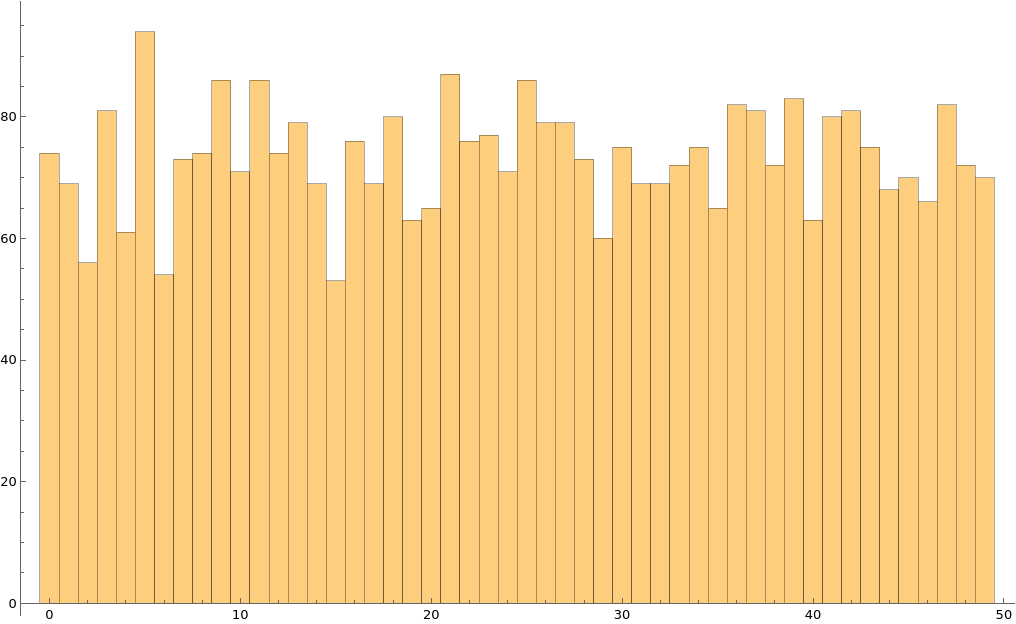
\includegraphics[width=0.75\textwidth]{figures/fig-lotto-bonusnumberuniform}
\caption{Histogram of 3,665 draws of the ``bonus number'' in Canada's 6/49 lotto, each draw being a number in $\{1,2,\dots,49\}$. Is the distribution uniform? Or is the lottery not fair?}
\end{figure}

So you have a reference distribution $\q\in\distribs{\ab}$ in mind. The first thing we will do is simplify the problem, and assume that $\q$ is not \emph{any} distribution, but \emph{the} uniform distribution $\uniformOn{\ab}$ over $\domain$.\marginnote{This is the \emph{uniformity testing} question, a special case of identity testing.} This will make our life easier. And while this seems like a big simplification, it turns out it is not! That is, any algorithm for \emph{uniformity testing} (the reference is $\uniformOn{\ab}$) can be used as a blackbox to solve the \emph{identity testing} (the reference is any $\q$), \emph{via} a reduction:
\begin{theorem}[Identity to uniformity reduction]
Suppose there is an algorithm $\Algo$ for uniformity testing, which takes $\ns=\ns(\ab,\dst,\errprob)$ \iid samples from the unknown distribution. Then there is an algorithm $\Algo'$ for identity testing over a domain of size $\ab$ to any fixed $\q\in\distribs{\ab}$, which takes $\ns=\ns(4\ab,\dst/4,\errprob)$ \iid samples from the unknown distribution. Moreover, $\Algo'$ is efficient if $\Algo$ is.
\end{theorem}
We will not prove this theorem here, but this essentially says that while uniformity and identity testing, they are basically equivalent (up to constant factors).

Now, all we need to solve is the \emph{uniformity testing} problem: given $\ns$ \iid samples from an unknown $\p$ over $\domain$, decide whether $\p=\uniformOn{\ab}$, or $\totalvardist{\p}{\uniformOn{\ab}} > \dst$ (and be correct with probability at least $1-\errprob$). Let's say $\errprob = 1/3$. How many samples $\ns$ would we have to take to solve this question?
\begin{itemize}
    \item $\ns = \bigO{\frac{\ab}{\dst^2}}$?
    \item $\ns = \bigO{\frac{\sqrt{\ab}}{\dst^2}}$?
    \item $\ns = \bigO{\frac{1}{\dst^2}}$?
    \item $\ns = \bigO{\frac{\log\ab}{\dst^2}}$?
\end{itemize}
In what follows, we will assume $\errprob=1/3$, since we can boost this to any $1-\errprob$ by a ``standard majority vote'' losing only an $O(\log(1/\errprob)$ factor in the number of samples $\ns$.\marginnote{Exercise: write down the details!}

\paragraph{A baseline: if we can learn, we can test.} The first claim is that the sample complexity of \emph{learning} is an upper bound on that of \emph{testing}: that is, one can always to do the following.
\begin{itemize}
    \item Learn $\p$ to total variation distance $\frac{\dst}{2}$ to obtain $\widehat{\p}$ such that $\totalvardist{\p}{\widehat{\p}} \leq \frac{\dst}{2}$ with probability at least $2/3$;
    \item Check (without taking any more samples) if $\totalvardist{\widehat{\p}}{\uniformOn{\ab}} \leq \frac{\dst}{2}$;
    \item Output $\yes$ if it is the case, $\no$ otherwise.
\end{itemize}
Since total variation distance is a metric, it satisfies the triangle inequality: so 
\begin{itemize}
    \item If $\p=\uniformOn{\ab}$, then $\totalvardist{\p}{\widehat{\p}} \leq \frac{\dst}{2}$ (with probability at least $2/3$);
    \item If $\totalvardist{\p}{\uniformOn{\ab}} > \dst$, then by the triangle inequality 
    \[
    \dst < \totalvardist{\p}{\widehat{\p}} 
    + \totalvardist{\widehat{\p}}{\uniformOn{\ab}}
    \]
    but by our learning guarantee the first term is at most $\dst/2$ (with probability at least $2/3$), so the second must be more than $\dst/2$.
\end{itemize}
This simple argument tells us that whatever we end up getting, we should do no worse than $\ns = O(\ab/\dst^2)$: since that is what the learning approach will get us.

\paragraph{But we can do better!} Alright, we can do $\ns = O(\ab)$ by learning: but again, here we only aim for \emph{one bit} of information. As it turns out, this allows us to do significantly better in terms of sample complexity:
\begin{theorem}
    \label{theo:testing:k}
    Testing uniformity of an unknown distribution $\p\in\distribs{\ab}$ to total variation distance $\dst$ (with success probability $2/3$) can be done with 
    \[
    \ns = \bigO{\frac{\sqrt{\ab}}{\dst^2}}
    \]\iid samples, using~\cref{algo:collision-based}. (Moreover, this is optimal for constant success probability.)
\end{theorem}
In terms of dependence on $\ab$, this is a \emph{quadratic} improvement over learning! Before giving (part of) the proof, you may wonder where this $\sqrt{\ab}$ comes from: at a high level, it comes from something we have seen before, the \emph{Birthday Paradox.}\marginnote{Why $\sqrt{\ab}$? Birthday Paradox.} Consider the distribution $\p$ which is uniform on an arbitrary subset of $\ab/2$ elements: it is easy to see that it is at total variation distance $1/2$ from $\uniformOn{\ab}$. But unless we take $\ns = \Omega(\sqrt{\ab})$ samples from $\p$, all we see is a sequence on unique elements from the domain, with zero collisions: which is entirely, and absolutely consistent with what we would see under the uniform distribution, too!

\begin{algorithm}[ht!]
  \begin{algorithmic}[1]
    \Require Multiset of $\ns$ \iid samples $x_1,\dots,x_\ns \in \domain$, parameters $\dst\in(0,1]$ and $\ab = \abs{\domain}$
    \State Set $\tau \gets \frac{1+2\dst^2}{\ab}$
    \State Compute \Comment{$O(\ns)$ time if $\domain$ is known}
    \[
        Z = \frac{1}{\binom{\ns}{2}} \sum_{1\leq s < t \leq \ns} \indic{x_s=x_t} = \frac{1}{\binom{\ns}{2}} \sum_{j\in\domain} \binom{\red{N}_j}{2}
    \] where $\red{N}_j \gets \sum_{t=1}^\ns\indic{x_t=j}$.
    \If{ $Z \geq \tau$ } \Return \no \Comment{Not uniform}
    \Else\ 
      \Return \yes \Comment{Uniform}
    \EndIf
  \end{algorithmic}
  \caption{\label{algo:collision-based}\sc Collision-Based Uniformity Tester}
\end{algorithm}
\begin{proof}[(Partial) proof of~\cref{theo:testing:k}]
\marginnote{\hl{We will only show here how to derive a (suboptimal) bound $\ns=\bigO{\sqrt{\ab}/\dst^4}$.}}
This idea that \emph{collisions} are important to test whether $\p$ is uniform is actually quite important, and the basis behind~\cref{algo:collision-based}. Namely, we will use the following facts: the first is what while TV distance is basically $\lp[1]$ distance between pmfs, the \emph{$\lp[2]$ distance is a good proxy for total variation distance}:
\begin{equation}
  \label{eq:relation:l1:l2:cs}
  \totalvardist{\p}{\uniformOn{\ab}} = \frac{1}{2}\normone{\p-\uniformOn{\ab}} \leq \frac{\sqrt{\ab}}{2}\normtwo{\p-\uniformOn{\ab}}
\end{equation}
the inequality being Cauchy--Schwarz. What this means is that
\begin{itemize}
    \item if $\totalvardist{\p}{\uniformOn{\ab}}>\dst$, then $\normtwo{\p-\uniformOn{\ab}}^2 > 4\dst^2/\ab$; while
    \item if $\totalvardist{\p}{\uniformOn{\ab}}=0$ then $\normtwo{\p-\uniformOn{\ab}}^2=0$ too.
\end{itemize}
So it is \emph{sufficient} to test with respect to $\lp[2]$ distance. What does that buy us? We have the very convenient fact, specific to the distance to the uniform distribution: for any distribution $\p$ over $\domain$,
\begin{equation}
  \label{eq:relation:collisionprob:distance:uniform}
  \normtwo{\p-\uniformOn{\ab}}^2 = \sum_{i=1}^{\ab} \Paren{\p(i)-\frac{1}{\ab}}^2  = \sum_{i=1}^{\ab} \p(i)^2-\frac{1}{\ab} = \normtwo{\p}^2-\frac{1}{\ab}\,,
\end{equation}
so combining the two we get that $\totalvardist{\p}{\uniformOn{\ab}}>\dst$ implies $\normtwo{\p}^2 > (1+4\dst^2)/\ab$.

\begin{remark}
  \label{rk:collision:probability}
  We have seen this quantity $\normtwo{\p}^2$ before! It is commonly known as the \emph{collision probability}\marginnote{It is easy to see, from~\cref{eq:relation:collisionprob:distance:uniform}, that among all probability distributions over a given support size $\ab$ the collision probability is minimised for the uniform distribution: indeed, $\normtwo{\p}^2 = \frac{1}{\ab}+ \normtwo{\p-\uniformOn{\ab}}^2 \geq \frac{1}{\ab}$.} of $\p$, due to the following fact: if $X,Y$ are \iid random variables distributed according to $\p$, then
  \begin{equation}
      \probaOf{X=Y} = \sum_{i\in\domain} \probaOf{X=i, Y=i} = \sum_{i\in\domain} \p(i)^2 = \normtwo{\p}^2
  \end{equation}
\end{remark}
In view of~\cref{eq:relation:collisionprob:distance:uniform}, a very natural idea is to estimate $\normtwo{\p}^2$, in order to distinguish between (i)~$\normtwo{\p}^2 = 1/\ab$ (uniform) and (ii)~$\normtwo{\p}^2 > (1+4\dst^2)/\ab$ ($\dst$-far from uniform). How to do that? We just saw that the probability that two independent samples from $\p$ take the same value (a ``collision'') is exactly $\normtwo{\p}^2$. Thus, 
an obvious approach is to take $\ns$ samples $x_1,\dots,x_\ns$, count the number of pairs that show a collision, and use that as an estimator $Z$ for $\normtwo{\p}^2$:\marginnote{Sanity check: why not just look at $\ns/2$ (independent) pairs of samples, and use them to estimate $\probaOf{X=Y}$?}
\begin{equation}
  \label{eq:def:z1}
    Z = \frac{1}{\binom{\ns}{2}} \sum_{1\leq s < t \leq \ns} \indic{x_s=x_t}\,.
\end{equation}
By the above, $\expect{Z} = \normtwo{\p}^2$. If we threshold $Z$ somewhere between (i) and (ii), at say 
\[
\tau\eqdef \frac{1+2\dst^2}{\ab}\]
we should be able to distinguish between our two cases and get a valid tester. But how large must $\ns$ be for this to work? \smallskip

Intuitively, we expect the test to work as long as the standard deviation of $Z$ (the ``noise'') is smaller than the gap between the expectations in our two cases (the ``signal''); that is,
\begin{equation}
  \label{eq:signal:to:noise}
      \sqrt{\var[Z]} \ll \Delta \expect{Z} = \frac{4\dst^2}{\ab}
\end{equation}
as this is the condition for the random fluctuations of our statistic $Z$ not to ``cross'' our threshold too often and lead to a wrong answer.

To make this quantitative, we can use Chebyshev's inequality, which requires us to bound $\var[Z]$. This is where things get tricky, since $Z$ is the sum of $\binom{\ns}{2}$ random variables which are \emph{not} pairwise independent.\footnote{Namely, the summands $\indic{X_s=X_t}$ in the definition of $Z$ are \emph{positively correlated}: 
\[
\cov(\indic{X_s=X_t},\indic{X_{s'}=X_{t'}}) \geq 0
\] and are only independent if $s,s',t,t'$ are all distinct.} 

We will only show here to derive a (suboptimal) bound $\ns=\bigO{\sqrt{\ab}/\dst^4}$:
\begin{align*}
  \var[Z] 
   &= \bEE{Z^2} - \bEE{Z}^2\\
   &= \frac{1}{\binom{\ns}{2}^2} \sum_{1\leq s < t \leq \ns}\sum_{1\leq s' < t' \leq \ns} \bEE{\indic{X_s=X_t}\indic{X_{s'}=X_{t'}}} - \normtwo{\p}^4
\end{align*}
To handle this last sum despite the lack of independence of the summands, we will break it in 3 groups depending on the cardinality of $\{s,t,s',t'\}$, which can be either 4 (all indices are distinct), 3 (one index is common to the two pairs), or 2 (both pairs of indices are the same).
\begin{itemize}
  \item In the first case, we have independence of the two indicator random variables, and 
  \[
    \bEE{\indic{X_s=X_t}\indic{X_{s'}=X_{t'}}} = \bEE{\indic{X_s=X_t}}\bEE{\indic{X_{s'}=X_{t'}}} = \normtwo{\p}^4.
  \]
  \item In the third case, the two indicator random variables are the same, and since $\indic{}^2=\indic{}$ we get
  \[
    \bEE{\indic{X_s=X_t}\indic{X_{s'}=X_{t'}}} = \bEE{\indic{X_s=X_t}} = \normtwo{\p}^2.
  \]
  \item The second case is the messiest one; still, one can verify that in this case $\indic{X_s=X_t}\indic{X_{s'}=X_{t'}}$ is 1 if, and only if, the three distinct samples corresponding to the 3 distinct indices among $s,t,s',t'$ take the same value, from which
  \[
    \bEE{\indic{X_s=X_t}\indic{X_{s'}=X_{t'}}} = \norm{\p}_3^3.
  \]
\end{itemize}
It remains to count how many summands of each type we have. Clearly, we have exactly $\binom{\ns}{2}$ summands of the third type; it is also not too hard to see that we have $\binom{\ns}{2}\binom{\ns-2}{2} = 6\binom{\ns}{4}$ summands of the first, and $6\binom{\ns}{3}$ of the second. (As a sanity check, $6\binom{\ns}{4}+6\binom{\ns}{3}+\binom{\ns}{2} = \binom{\ns}{2}^2$, so all our summands are accounted for.)

Getting back to our variance computation, this yields
\begin{align}
  \var[Z] 
   &= \frac{1}{\binom{\ns}{2}^2} \Paren{ 6\binom{\ns}{4}\normtwo{\p}^4+6\binom{\ns}{3}\norm{\p}_3^3+\binom{\ns}{2}\normtwo{\p}^2 } - \normtwo{\p}^4 \notag\\
   &= \frac{1}{\binom{\ns}{2}^2} \Paren{ \Paren{6\binom{\ns}{4} - \binom{\ns}{2}^2}\normtwo{\p}^4+6\binom{\ns}{3}\norm{\p}_3^3+\binom{\ns}{2}\normtwo{\p}^2 } \label{eq:collisionbased:loose}\\
   &\leq \frac{4}{\ns}\norm{\p}_3^3+\frac{4}{\ns^2}\normtwo{\p}^2 \notag\\
   &\leq \frac{4}{\ns}\bEE{Z}^{3/2}+\frac{4}{\ns^2}\bEE{Z}  \notag
\end{align}
first using that $6\binom{\ns}{4} < \binom{\ns}{2}^2$ to discard a negative term, then that $\ns \geq 2$ to get a simpler-looking upper bound on binomial coefficients, and finally writing $\norm{\p}_3 \leq \normtwo{\p}$ by monotonicity of $\lp[p]$ norms.

\begin{itemize}
    \item In the case when $\p=\uniformOn{\ab}$ (often called the \emph{completeness} case), we need to control the probability that $Z$ crosses our threshold $\tau \eqdef \frac{1+2\dst^2}{\ab}$, that is
\[
    \bPr{Z \geq \tau} = \bPr{Z \geq (1+2\dst^2)\bEE{Z}} \leq \bPr{Z \geq (1+\dst^2)\bEE{Z}}
\]
\item in the ``far'' case (often called the \emph{soundness}\index{soundness} case), we want to control
\[
    \bPr{Z < \tau} \leq \bPr{Z < \frac{(1-\dst^2)(1+4\dst^2)}{\ab}} \leq \bPr{Z < (1-\dst^2)\bEE{Z}}
\]
using first that $(1-\dst^2)(1+4\dst^2) \geq 1+2\dst^2$ (for $\dst\leq 1/2$), and then the fact that in the ``far'' case $\bEE{Z} > \frac{1+4\dst^2}{\ab}$.
\end{itemize}

To control our probability of error in both cases, it is thus sufficient to upper bound $\bPr{\abs{Z-\bEE{Z}} \geq \dst^2\bEE{Z}}$; by Chebyshev's inequality (\cref{theo:chebyshev}), this is at most
\begin{align*}
    \bPr{\abs{Z-\bEE{Z}} \geq \dst^2\bEE{Z}}
    &\leq \frac{\var[Z] }{\dst^4\bEE{Z}^2} \\
    &\leq \frac{4}{\dst^4\ns\bEE{Z}^{1/2}}+\frac{4}{\dst^4\ns^2\bEE{Z}} \\
    &\leq \frac{4\sqrt{\ab}}{\dst^4\ns}+\frac{4\ab}{\dst^4\ns^2}
\end{align*}
which is at most $1/3$, as desired, for $\ns \geq \frac{13\sqrt{\ab}}{\dst^4}$. (For the third inequality, we relied on the fact that $\bEE{Z} = \normtwo{\p}^2 \geq 1/\ab$ (cf. \cref{rk:collision:probability}).)
\end{proof}
\emph{The algorithm can be shown to work even for $\ns=O(\sqrt{\ab}/\dst^2)$, but this require a much more careful variance analysis.}
As mentioned above, this $2/3$ can be boosted to $1-\errprob$, for sample complexity
$\bigO{\frac{\sqrt{\ab} \log(1/\errprob)}{\dst^2}}$.
\paragraph{Yet we can do better!} To conclude this lecture: we can do even better! The actual, optimal sample complexity of uniformity testing \emph{has} been pinpointed,\cite{DGPP:18} and it is (perhaps surprisingly) a bit strange.
\begin{theorem}
    \label{theo:testing:k:refined}
    Testing uniformity of an unknown distribution $\p\in\distribs{\ab}$ to total variation distance $\dst$ (with success probability $1-\errprob$) can be done with 
    \[
    \ns = \bigO{\frac{\sqrt{\ab\log(1/\errprob)} + \log(1/\errprob)}{\dst^2}}
    \]\iid samples. (Moreover, this is optimal.)
\end{theorem}
The proof is outside the scope of this lecture, but note the rather strange dependence on $\errprob$! This is quite useful for very, very small $\errprob$.
%\section{Parameter estimation?}

%Everything is complicated
%Tolerant testing/parameter estimation reduction (proof in tutorial)
\paragraph{A concluding remark.} We may be tempted to consider a more robust version of testing: return \yes when $\totalvardist{\p}{\uniformOn{\ab}} \leq \dst_1$, and \no when $\totalvardist{\p}{\uniformOn{\ab}} > \dst_2$, for two arbitrary input parameters $0 \leq \dst_1 < \dst_2 \leq 1$. Unfortunately, this turns out to be a \emph{much} harder problem, which (even when $\dst_1,\dst_2 = \Theta(1)$), requires $\ns = \bigTheta{\frac{\ab}{\log\ab}}$ samples!\cite{VV:11:stoc}


% Add exercise on tolerant testing. v. distance approximation?